
\chapter{Introduction}

In recent human history there has been tremendous progress in sciences and the benefits can be coupled with the increase in life expectancy. About 150 years ago an average person would live up to 30 years, but now we're expecting to reach an average age of 70 years, and better prospects are in high-income countries like U.K. or Japan, as seen in Figure \ref{fig:life_expectancy}. Most of the technologies played a role in the increased welfare of the world population, but the advances in healthcare and our biological understanding had directly improved life expectancy. As cancer is typically a disease of ageing and as the world's population grows older a side effect is that more people get cancer in modern times.

In an article titled "Is the world making progress against cancer?"\cite{World_in_Data_undated-gc}\footnote{I found the graphs from Our World in Data to be useful in understanding the scale of cancer and they have more graphs dedicated to cancer on their website\cite{Roser2015-qb}. }, Dr Max Roser gives an overview of humanity's progress on the disease. It is expected, that as both the population and life expectancy grow, there will be more people predisposed to cancers, and this is represented by the green line in Figure \ref{fig:cancer_death}; the cancer death rate increased to 66\% in 2017 from 1990. The red line is the cancer death rate per 100,000 and that only increased 17\% which means that if the World's population will have they stayed the same as in 1990, the cancer deaths will increase only a quarter. If the age is standardized then it can be seen that the death rate drops to -15\%. Therefore, Figure \ref{fig:cancer_death} tells us that there has been some progress in solving cancer, but there is a need for more concentration of effort as life expectancy continues to increase.

\begin{figure}[!htb]
    \centering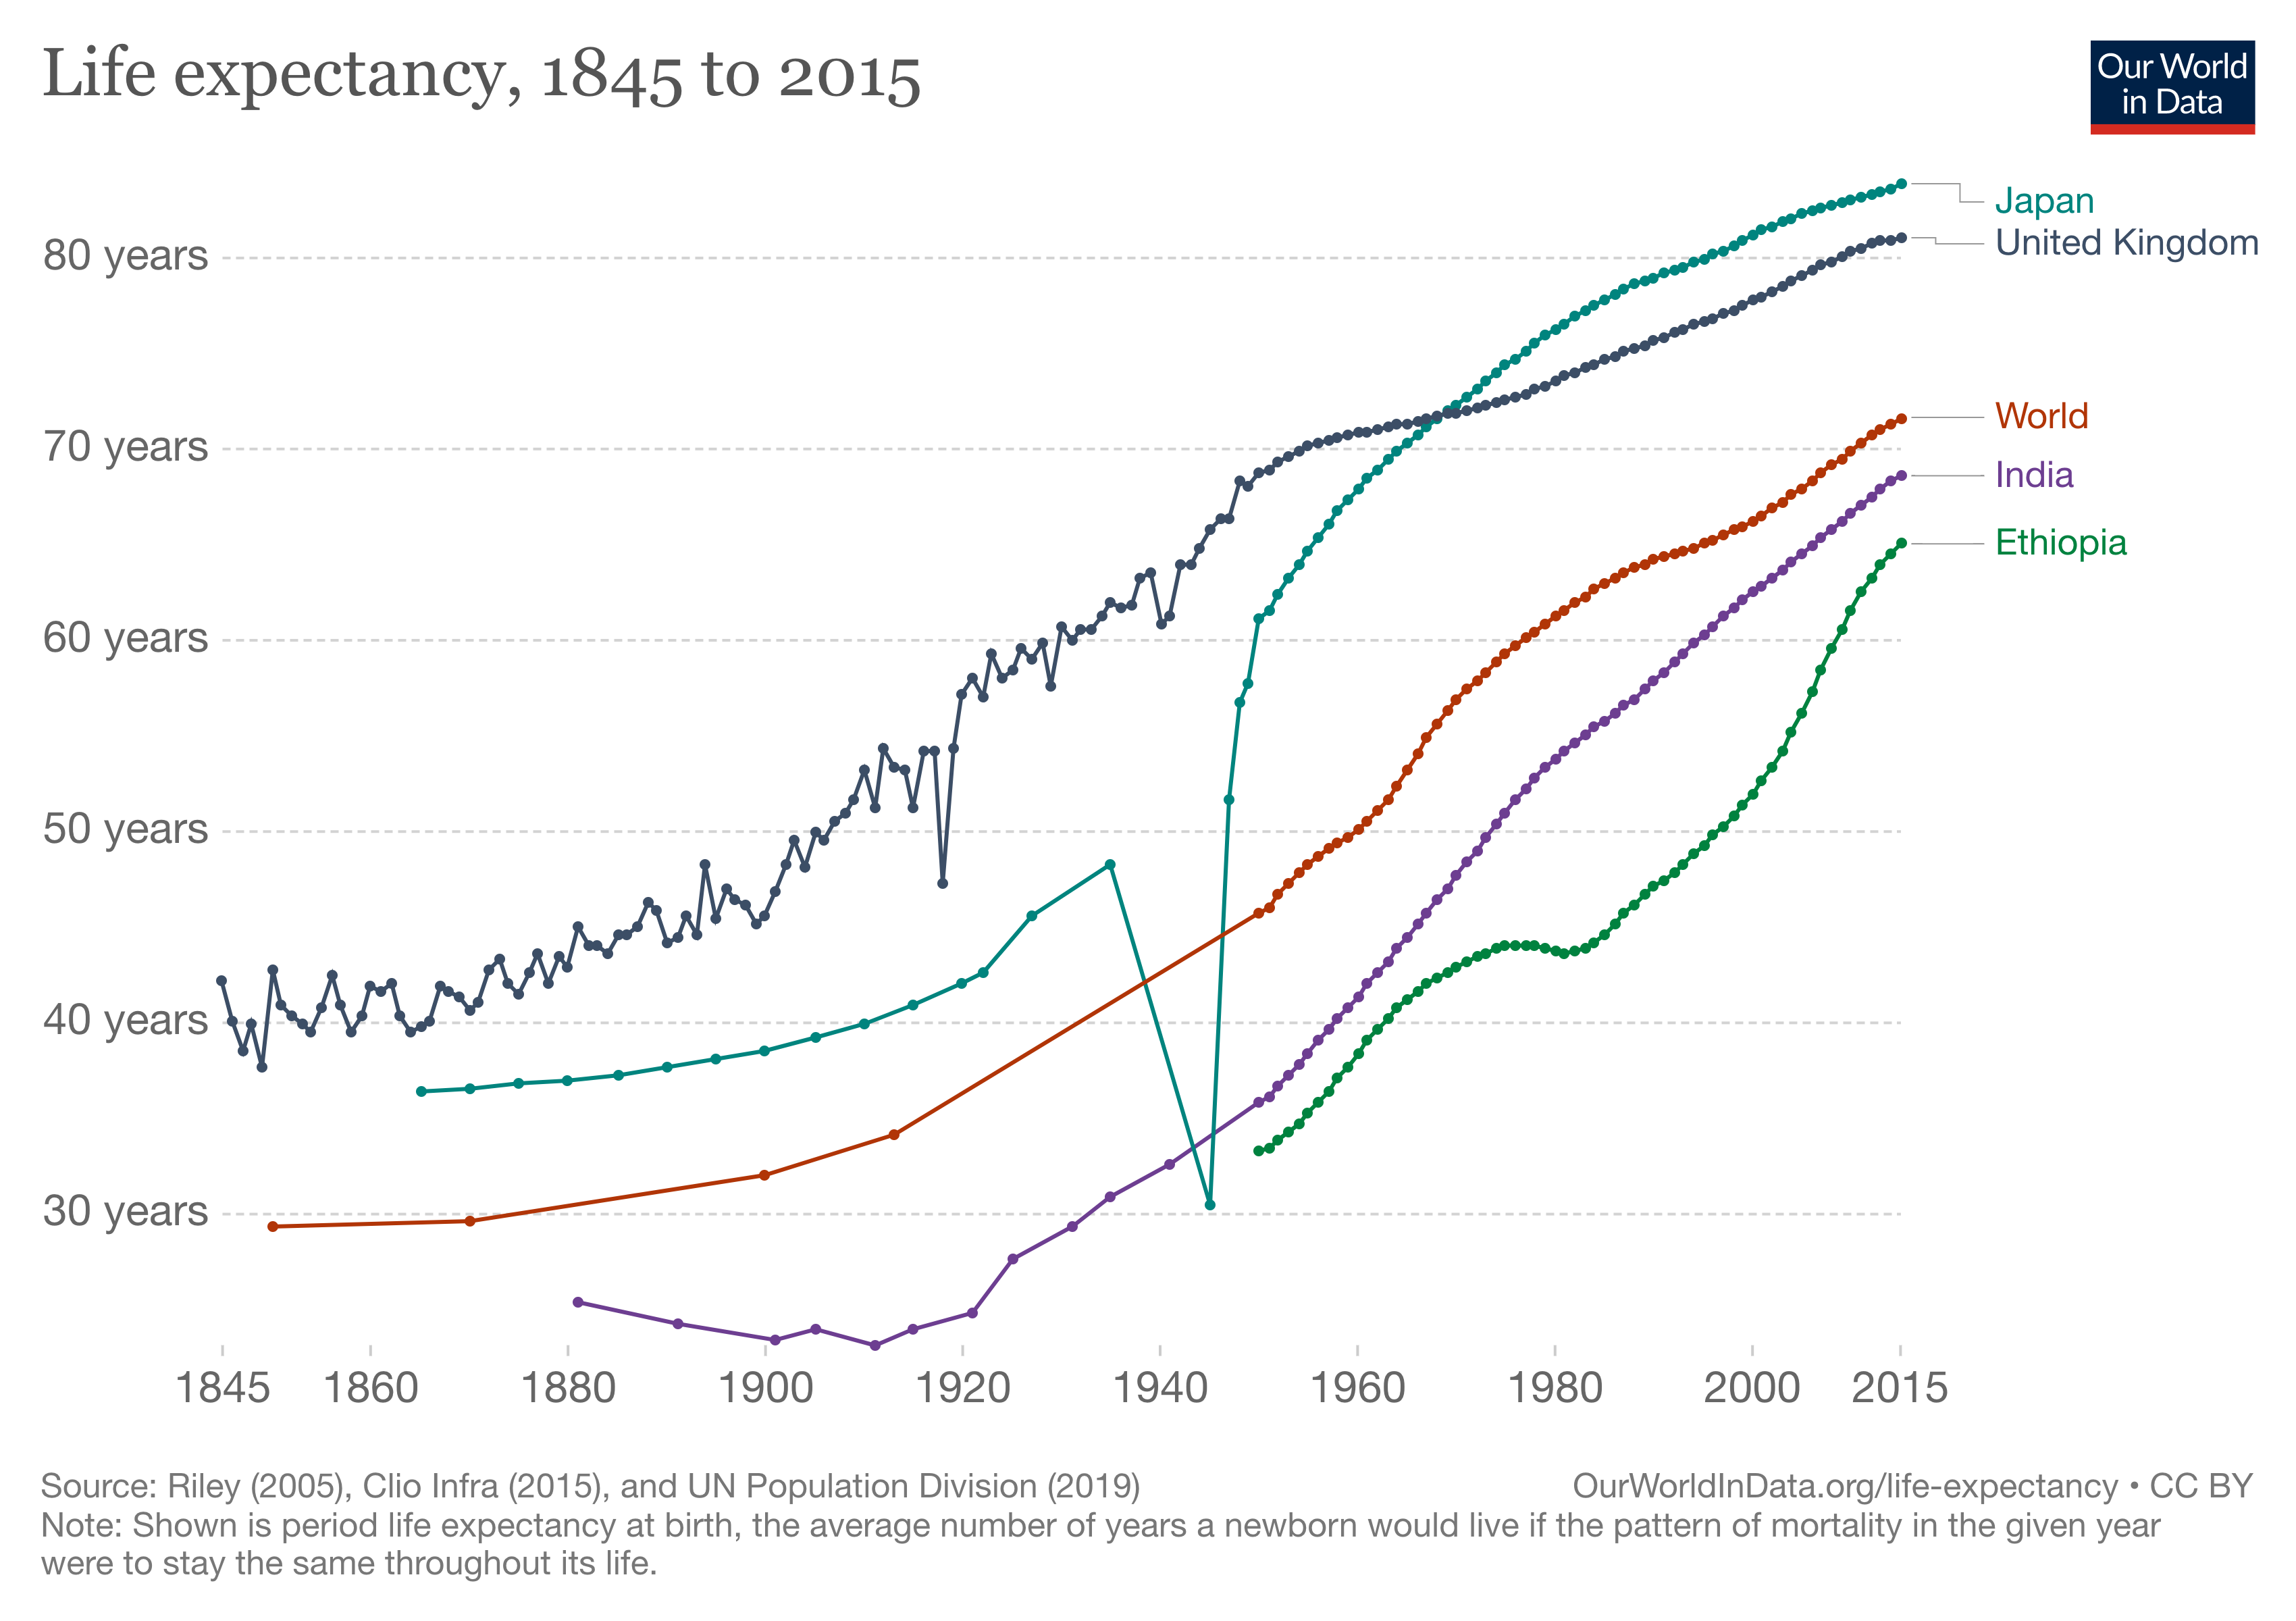
\includegraphics[width=1.0\textwidth,height=0.3\textheight,keepaspectratio]{Images/life-expectancy.png}
      \caption{Life expectancy according to World in Data between 1845 - 2015\cite{World_in_Data_undated-no}}
      \label{fig:life_expectancy}
\end{figure}


According to Cancer Research UK\cite{Cancer_Research_UK2015-cf}, the bladder is the 10th leading cause of death, it accounts for 3\% of all deaths in the U.K. and 56\% of incidence is in people older than 75. Almost half (52.6\%) of the people diagnosed with bladder cancer survive for more than five years, and 46.4\% for more than ten years. 

This project focuses on understanding better the mechanism of cancer from genomic data, which includes both mutation and gene expression. The initial focus will be on bladder cancer as the Jack Birch Unit (JBU) holds knowledge on the normal behaviour of the tissue which enables the integration of domain knowledge into the computational models. Furthermore, there are publicly available datasets on Bladder Cancer such as \acrfull{tcga}\cite{Tcga2018-sj} and Uromol dataset\cite{Lindskrog2021-ov, The_European_Genome-phenome_Archive_undated-pz}.

The purpose of this report is to introduce the reader to the research in multi-omics (Chapter \ref{s:lit:multi-omics}) which itself can be split in multiple areas: Consensus subtyping \& the user of Transcriptomic data (Section \ref{s:lit:rnaSeq}), processing mutations data (Section \ref{s:lit:mutations}), combined approaches (Section \ref{s:multi-view}) and Deep Learning (\ref{s:lit:dl_genomics}). The relevant concepts throughout  Chapter \ref{s:lit:multi-omics} are described in the subsections from Chapter \ref{s:lit:computational}. This document finishes with a discussion and the Aims \& Goals (\ref{s:aims}) of the project. In addition, as part of the submission, a Gantt chart is included that describes the project's plan for the upcoming year. 

\begin{figure}[!htb]
    \centering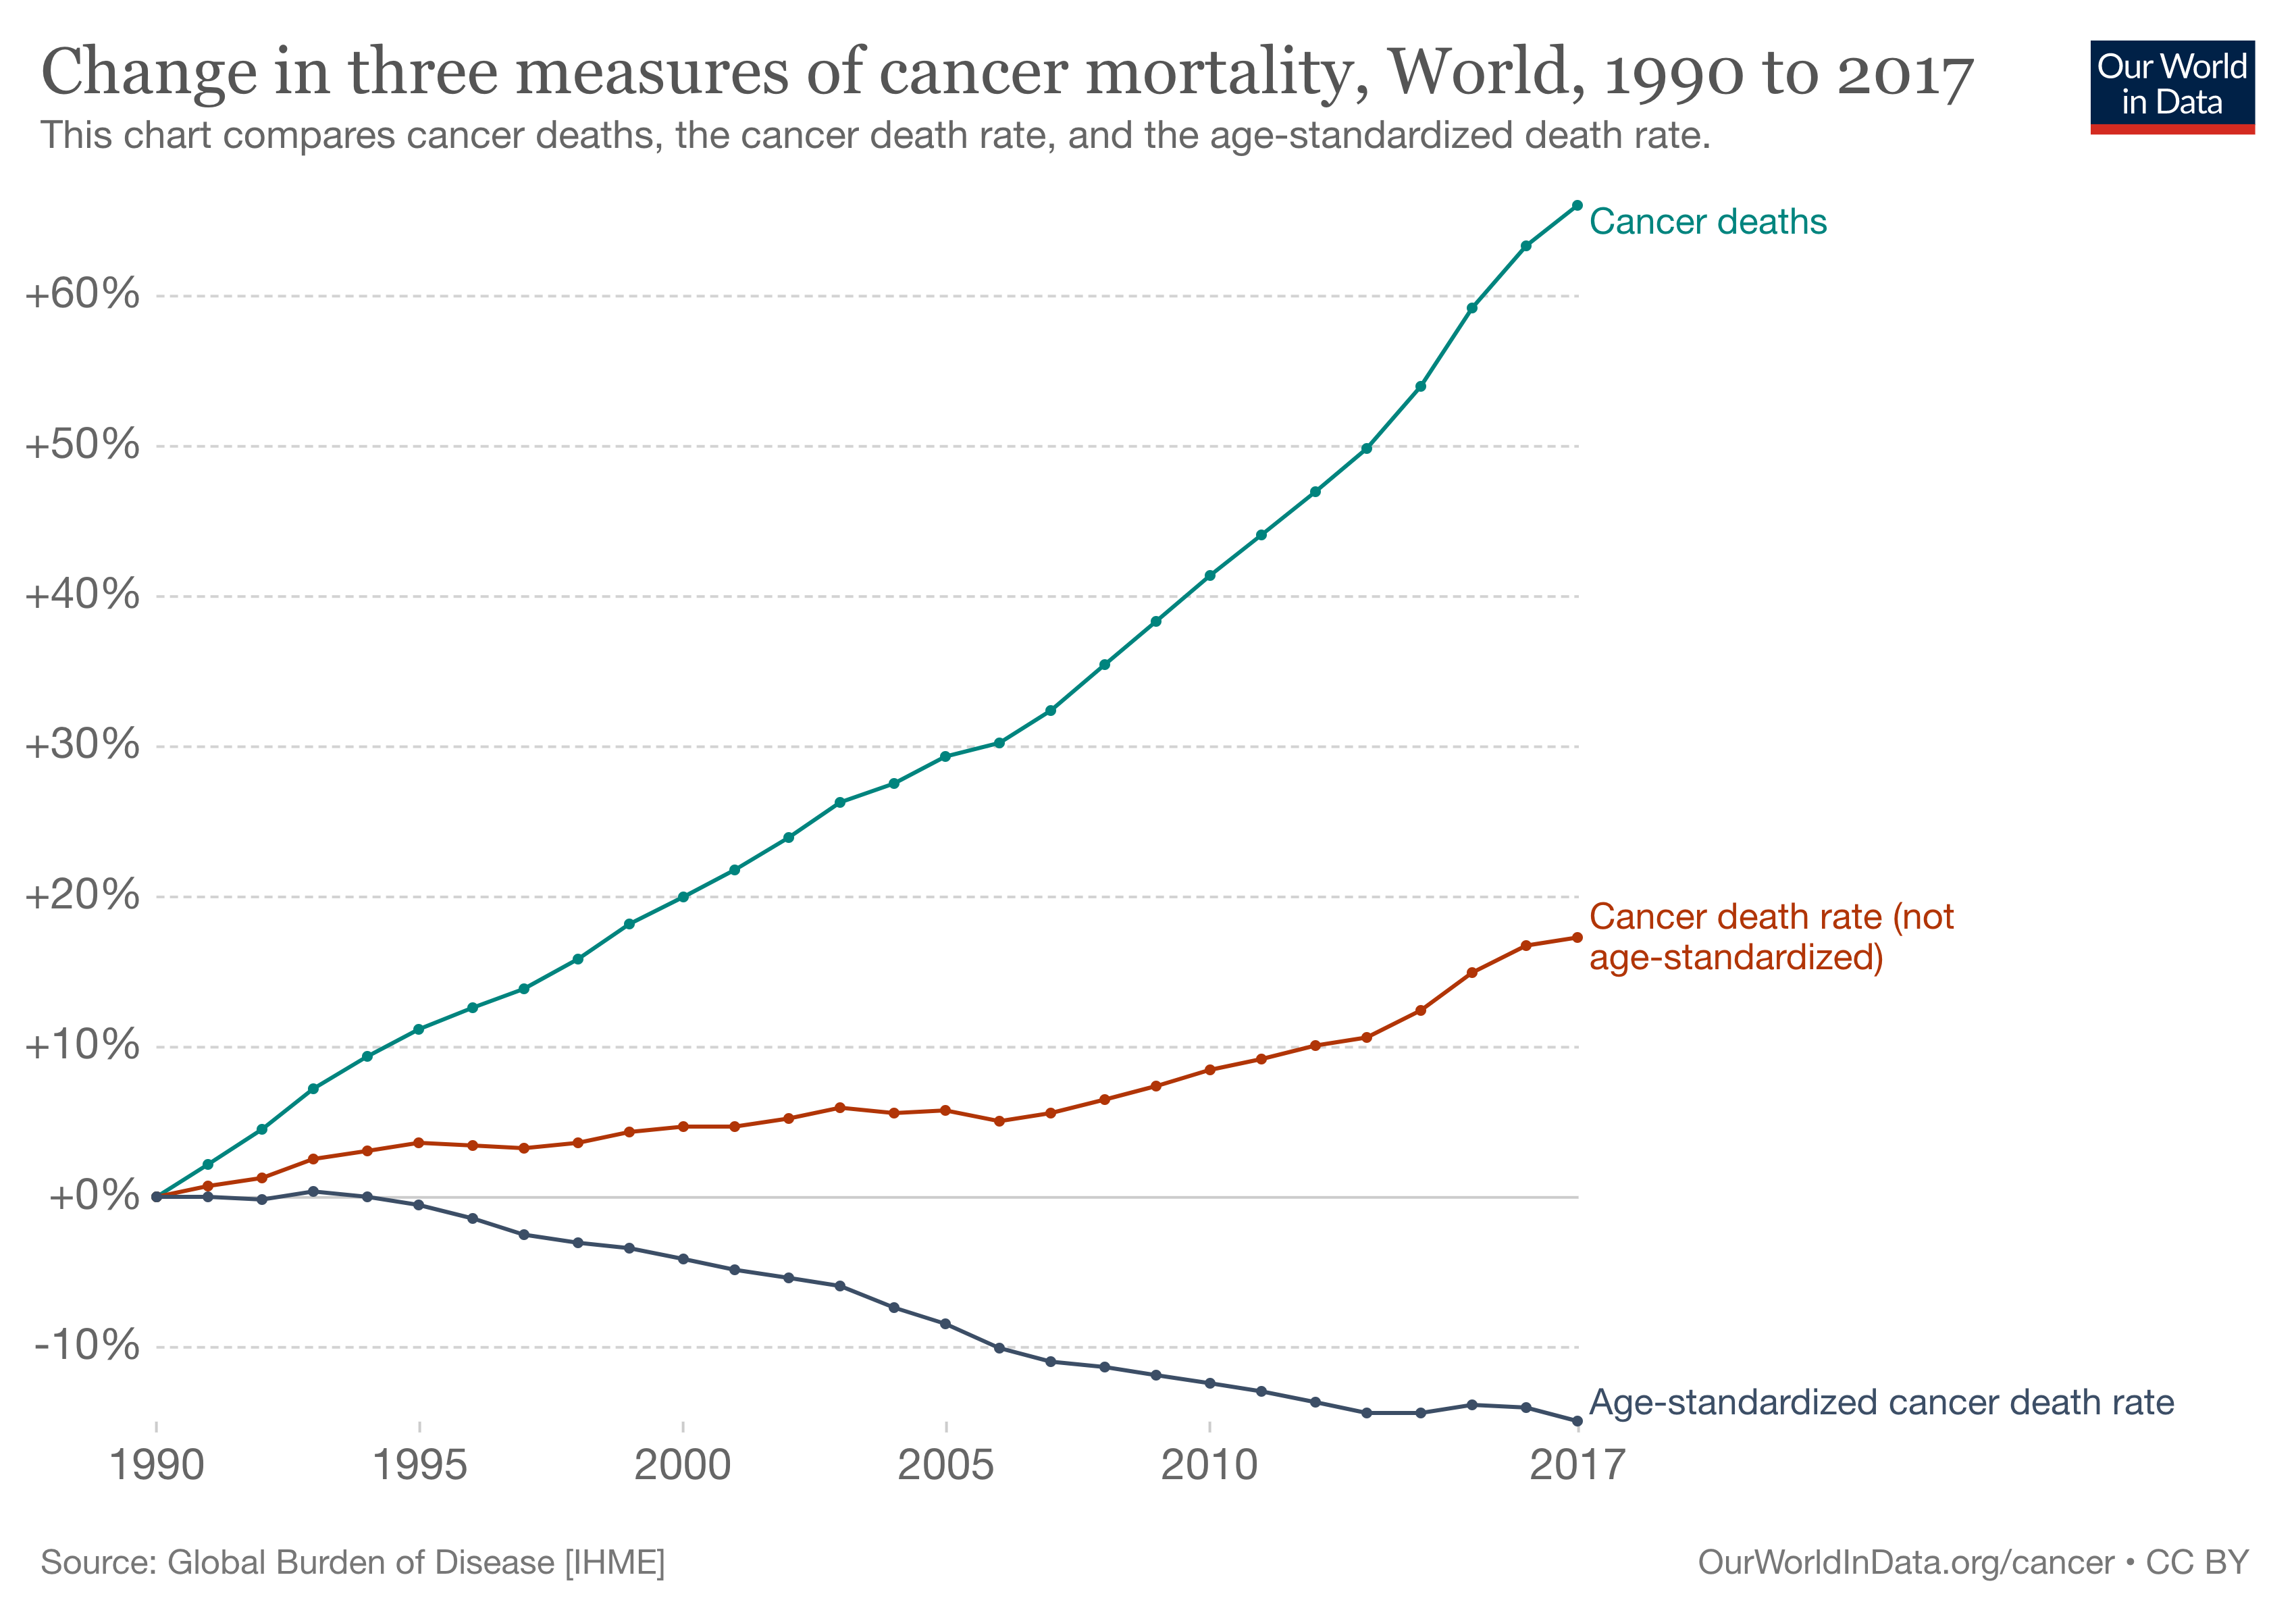
\includegraphics[width=1.0\textwidth,height=0.3\textheight,keepaspectratio]{Images/cancer-deaths-rate-and-age-standardized-rate-index.png}
      \caption{Changes in cancer mortality between 1990 and 2017. \cite{World_in_Data_undated-gc}}
      \label{fig:cancer_death}
\end{figure}


\newpage

\subsection{Overview of the cancer stratification}

\begin{itemize}
    \item Introducing the problem of cancer stratification and why it is important
    \item Present bladder cancer, muscle invasive bladder cancer (MIBC) and non-muscle invasive bladder cancer (NMIBC)
\end{itemize}

\subsection{Motivation}

\begin{itemize}
    \item Introduce the different classifiers to stratify MIBC (e.g., Lund, TCGA, consensus)
    \item Limitations of the current approaches
    \begin{itemize}
        \item Performing separate analysis for each data type and then combined the outputs 
        \item If there are integrated at the computational stage (iCluster) these are hard to interpret and find which genes contributed to each subtype.
    \end{itemize}
    \item Technological progress    
    \begin{itemize}
        \item The RNAseq data becomes cheape
    \end{itemize}
\end{itemize}


Explain the potential of the network approaches to integrate the data.
\begin{itemize}
    \item A model estimation for genes interactions through node’s edges
    \item The edges can be modified to include other information such as mutations.
    \item It can be interpreted and understood 
    Visualisation
\end{itemize}

Challenges with the network approaches
\begin{itemize}
    \item Representation based on genes.
    \item Methods less developed to interpret them. 
\end{itemize}

\subsection{Hypothesis} 

Combining multiple data types at the computational stage will improve cluster stratification. This in turn it will enable a greater understanding of the cancer's biology and potentially will lead to better treatments.


\subsection{Novelty} 


\begin{itemize}
    \item Only RNAseq data
    \begin{itemize}
        \item Basal split of the TCGA dataset using K-means 
        \item Aligned with INF$\gamma$ experiments
    \end{itemize}
    \item Combination of computational approach and biological healthy data
    \begin{itemize}
        \item Modifying a network's weights to integrate other data types is something that hasn’t been done before nor the modifications of number of connections with the goal to stratify a cancer 
        \item Using healthy data to generate a network and then subtype the tumour is also a new approach to stratify a cancer
    \end{itemize}
\end{itemize}


Contribution to knowledge. There are several Python scripts developed throughout the project to aid the data exploration and analysis, the biological interpretation and visualising other data types on Gephi (network visualiser):
\begin{itemize}
    \item The scripts developed to analyse networks
    \item The pipelines developed to analyse the data
\end{itemize}


\subsection{Datasets used} 

\begin{itemize}
    \item Introduce the datasets used: TCGA, JBU's datasets on healthy tissue
    \item Describe what type data we have: RNAseq and WES
\end{itemize}


\subsection{Thesis overview } 


The goal of this section is to briefly describe each chapter and highlight the important findings in each.

\begin{itemize}
    \item Literature Review
    \item Clustering Analysis
    \item iCluster (?)
    \item Network I - PGCNA
    \begin{itemize}
        \item PGCNA standard vs the clustering analysis
        \item PGCNA with mutations
    \end{itemize}
    \item Network II - perturbations
    \begin{itemize}
        \item Constructing a network from perturbations
    \end{itemize}
\end{itemize}